\documentclass[conference]{IEEEtran}
\usepackage{times}

% numbers option provides compact numerical references in the text. 
\usepackage[numbers]{natbib}
\usepackage{multicol}
\usepackage[bookmarks=true]{hyperref}
\usepackage{graphics} % for pdf, bitmapped graphics files
\usepackage{graphicx}
\usepackage{amsmath,amssymb,latexsym,float,epsfig,subfigure}
\usepackage{amsmath} % assumes amsmath package installed
\usepackage{amssymb}  % assumes amsmath package installed
\usepackage{lipsum}
\usepackage[export]{adjustbox}
\usepackage[normalem]{ulem} % underline
\usepackage{wrapfig}
\usepackage{multirow}
\usepackage{balance}
\usepackage{color}
\usepackage{url}
\newcommand{\argmax}{\arg\!\max}
\newcommand{\norm}[1]{\left\lVert#1\right\rVert}
\pdfinfo{
   /Author (Homer Simpson)
   /Title  (Robots: Our new overlords)
   /CreationDate (D:20101201120000)
   /Subject (Robots)
   /Keywords (Robots;Overlords)
}

\begin{document}

% paper title
\title{Mode switch assistance maximizing confidence disambiguation}

% You will get a Paper-ID when submitting a pdf file to the conference system
%\author{Deepak Gopinath and Brenna D. Argall}

\author{\authorblockN{Deepak Gopinath}
\authorblockA{Department of Mechanical\\Engineering,
Northwestern University\\
Evanston, Illinois 30332\\
Email: deepakedakkattilgopinath2015\\@u.northwestern.edu}
\and
\authorblockN{Brenna D. Argall}
\authorblockA{Department of Mechanical\\Engineering,
		Northwestern University\\
		Evanston, Illinois 30332\\
		Email: brenna.argall@northwestern.edu}}


% avoiding spaces at the end of the author lines is not a problem with
% conference papers because we don't use \thanks or \IEEEmembership


% for over three affiliations, or if they all won't fit within the width
% of the page, use this alternative format:
% 
%\author{\authorblockN{Michael Shell\authorrefmark{1},
%Homer Simpson\authorrefmark{2},
%James Kirk\authorrefmark{3}, 
%Montgomery Scott\authorrefmark{3} and
%Eldon Tyrell\authorrefmark{4}}
%\authorblockA{\authorrefmark{1}School of Electrical and Computer Engineering\\
%Georgia Institute of Technology,
%Atlanta, Georgia 30332--0250\\ Email: mshell@ece.gatech.edu}
%\authorblockA{\authorrefmark{2}Twentieth Century Fox, Springfield, USA\\
%Email: homer@thesimpsons.com}
%\authorblockA{\authorrefmark{3}Starfleet Academy, San Francisco, California 96678-2391\\
%Telephone: (800) 555--1212, Fax: (888) 555--1212}
%\authorblockA{\authorrefmark{4}Tyrell Inc., 123 Replicant Street, Los Angeles, California 90210--4321}}


\maketitle

\begin{abstract}
The abstract goes here.
\end{abstract}

\IEEEpeerreviewmaketitle

\section{Introduction}

Assistive and rehabilitation devices such as powered wheelchairs, robotic arms and myoelectric prosthesis play an important role in the lives of people with motor impairments. These devices help to increase their ability to perform activities of daily lives and reduce their dependence on caretakers and is crucial to revolutionizing the way they interact with society. As the field of assistive robotics progresses rapidly, the devices themselves become more capable and dextrous and as a result more complex, high dimensional and harder to control. 

A possible paradigm for control of such high dimensional devices is one in which the human directly controls the motion via a control interface. The confounding factor is that the more severe a person's motor impairment, the more limited are the control interfaces available to them to operate. These interfaces (for example, head arrays and Sip-N-puffs) are lower in dimensionality and bandwidth and usually require more mode switches for successful task completion. Thus, a greater need for sophisticated assistive devices is paired with a diminishing ability to control their additional complexity. 

Due to the dimensionality mismatch between the control interface and the robotic device, control interfaces can only operate in \textit{modes} which correspond to different parts of the control space. Typically, the more limited the control interface is, the greater number of modes there are. In order to have full control of the robot the user will have to switch between the difference partitions of the control space and this is known as \textit{mode switching}. 

It has been established that mode switching is expensive and as a result task performance is degraded. Furthermore, it adds to the cognitive and physical burden as each of these mode switches requires the user to shift their attention from the task to performing the mode switch. The introduction of \textit{shared autonomy} to these systems helps to alleviate and address some of these issues by letting the system take responsibility to some extent, thereby reducing the human effort in achieving a goal. 

Shared autonomy paradigms in assistive robotics can be broadly classified into two categories: \textit{heirarchical} and \textit{blending}. An example of a \textit{hierarchical} assistance system is one in which the user acts as an \textit{indicator} of goals and the robot executes the motion autonomously. In a \textit{blending} based assistance paradigm, the robot and the human work in the same control space (for example, velocity blending in Cartesian space) and usually the final control command issued to the robot is a blended sum of an autonomous robot policy and the control command issued by the human. 
\begin{figure}[t]
	\centering
	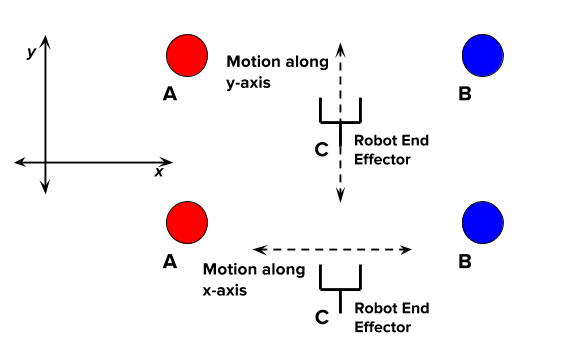
\includegraphics[width = 1.0\hsize]{./figures/DE.png}
	\caption{A and B indicate two point goal locations. The robot end effector is at location C. It is clear that any motion of the end effector along the y-axis will not help the system to disambiguate between the two goals; that is, the motion is not legible. However, if the human moves the robot along the x-axis, the system will be able to infer the goal immediately based on the direction in which the robot moves. }
	\label{DE}
\end{figure}
In this paper, we develop a mode switching assistance paradigm that augments an underlying blending-based shared control system for an assistive robotic arm. For blending, the assistance provided by the robot is regulated by the robot's ability to estimate user intent confidently and accurately and it is very unlikely that the robot will be able to determine this with a 100\% accuracy.  Therefore in the literature to date, the blending factor is usually a function of a confidence metric. This confidence metric is the system's confidence in its own estimate of human intent and is usually a function of the human control command, the autonomous policy, robot pose, goal locations, \textit{et cetera}. This implies that human control actions have a direct impact on the confidence measure. 

However, it can be the case that certain actions by the human might carry more information than others and better express the human intent which can then help the robot to draw useful and correct inferences more easily. That is, certain human actions are more \textit{legible} than others. However, the control commands that a human can generate is limited by the control mode in which he/she is operating. 

The concept of \textit{legibility} is typically used in the domain of human-robot interaction (HRI) as applied to robot motion. A \textit{legible} motion in this context is one which will help the observer (usually the human) decipher the intent behind the robot's action more \textit{quickly} and \textit{confidently}. In our work, we propose a paradigm of \textit{inverse legibility} in which the roles are switched and the human generated action helps the \textit{robot} to infer human intent confidently and accurately. \textbf{[Can there be a concept of bilateral legibility? The human knows the goal. And therefore has a model for what a predictable motion is. If the robot indeed performs that predictable motion, there is an agreement between the expectation and what really happened. That is, the robot motion becomes legible.]}

Consider the example illustrated in Figure~\ref{DE}. In this 2D world, a human control command issued along the $x$ dimension is more \textit{intent expressive} and helps the robot to provide the right kind of assistance more quickly and confidently. With the mode switching assistance scheme developed in this work, we hope to elicit more legible human control commands by placing the user control in those modes with \textit{maximum confidence disambiguation} between the various goals in the scene. 

The commonplace notion in human-robot interaction and especially in assistive robotics is that ``help'' is provided solely by the robot. In addition to eliciting more legible motion from the human, we also seek to explore and exploit the underlying synergies in human robot interaction to facilitate more seamless and efficient task execution. The idea of \textit{``people helping robots helping people''} is key here and by requiring the human to operate in a mode that will potentially help the robot in deciphering the intent the human, in some sense, helps the robot to perform more effectively.
It is possible that in some cases such a mode might not be the most ideal mode \textit{for} the human to operate in due to personal preferences. However, if the human agrees to compromise a little bit and provides ``hints" and ``nudges" the robot in the right direction, the overall performance gain will likely outweigh the slight sub-optimality due to the ``wrong'' mode. 

In Section \ref{RW} we present an overview of the relevant research in the area of shared control in assistance systems focusing on mode switching, legibility and synergies in HRI. Section \ref{ALGO} describes the mathematical formalism for the algorithm and the metric used for confidence disambiguation. The study methods, tasks and metrics are discussed in Section \ref{EXP}. In Section \ref{RES} we present the preliminary results from our pilot study and discussions followed by conclusions in Section \ref{CON}

\section{RELATED WORKS}\label{RW} 

Shared control assistance paradigms help to offload cognitive and physical burden~\cite{volosyak2005rehabilitation} without requiring the user to relinquish complete control and are usually preferred over fully autonomous assistive robotic systems for reasons of both robustness and user satisfaction. One possible way to control high dimensional assistive devices such as robotic arms is to partition the control space (often 6D for a robotic arm) into subsets called \textit{modes} and have the user control one mode at a time using control interfaces such as joysticks~\cite{tsui2008development}, head arrays and sip-and-puffs. This is known as \textit{modal control}.

Herlant \textit{et al.}~\cite{herlant2016assistive} assesses the difficulties faced by users when they operate assistive devices using \textit{modal control}. In their work they report that a significant number of users found \textit{mode switching} to be slow and burdensome. The cognitive burden of shifting focus (also known as \textit{task switching})  from the task at hand to mode switches can result in a significant decrease in task performance regardless of the control modality~\cite{monsell2003task}. 

 A time-optimal mode switch assistance paradigm evaluated on a simulated 2D robot provides insight into the fact that even a simple time optimal automatic mode switching system can significantly improve user satisfaction while maintaining the quality task performance~\cite{herlant2016assistive}.  Another study~\cite{gopinath2017human} found that it is not always the case that users are trying to optimize for time or effort during task execution. However, our present system therefore does not make \textit{a priori} assumptions regarding the optimizing principles at work when a user operates a robot.

Legibility and predictability of \textit{robot motion} has been thoroughly investigated~\cite{dragan2013legibility,dragan2013generating}, and different methods for generating legible robot motion have been proposed by Dragan \textit{et al}. We apply similar concepts of legibility however to the \textit{human control} commands, such that the intent expressed in the human command is clear \textit{to} the robot. Our assistance scheme is intended to bring out a more legible intent-expressive control command from the human, so that the system is able to infer the correct goal more confidently. 
%In most cases the human knows beforehand what goal he/she is going for and therefore the motion generated by the human is usually \textit{predictable}.
As long as the confidence measure used in the underlying blending paradigm captures the predictable aspect of human generated robot motion, the mode switching assistance proposed by us will place user control in that mode which can provide maximal confidence disambiguation thereby improving the legibility.

Also related to our work is the idea of mutual cooperation between humans and robots and the underlying synergies that are crucial for successful human-robot interaction. Sorokin \textit{et al.}~\cite{sorokin2010people} proposes a framework in which for human-robot interaction in which humans provide semantic information and judgments about the environment to the robot which then utilizes them to improves its own capabilities. Rosenthal et al. proposes a \textit{symbiotic} human robot interaction scheme which aims to overcome perceptual and cognitive limitations that robots might encounter while still allowing the robots to help humans as well~\cite{rosenthal2010effective}. 

%2-4 works which investigates what legibility means, proposes ways to generate legible robot motion. In all these works, the goal is to make the motion more legible for the human. In our system, we want the human to move the robot in a way that the intent is more legible FOR the system. That is the roles are reversed. Since the human knows beforehand what goal he/she is going after the motion generated by the human is usually predictable. As long as the confidence measure is able to capitalize on this predictability, the system can force the human to generate legible motions by requiring them to operate in those modes which can provide maximal confidence disambiguation. The notion of a confidence mediated blending paradigm is formalized in other Dragan paper. 
%
%Discuss works which formalizes legibility. Talk about how in the present work we are flipping roles and concerned more about the legibility of human's actions (which causes robot motion). Dragan et al. formalizes and investigates legibility and predictability of robot motion. Their paper's concern was primarily to make a robot's motion more legible for the human who will the observer. In the present work, we use the principle of legibility, except that the robot and the human switch roles. The human controls the robot motion via a control interface and robot is the ``observer'' and the system seeks to elicit to legible indicators \textit{from} the human in order to provide more effective assistance.

%Discuss works which emphasize two way interaction for more gain. Look into this a little more closely. Synergy related work. 
\begin{figure*}[t]
	\centering
	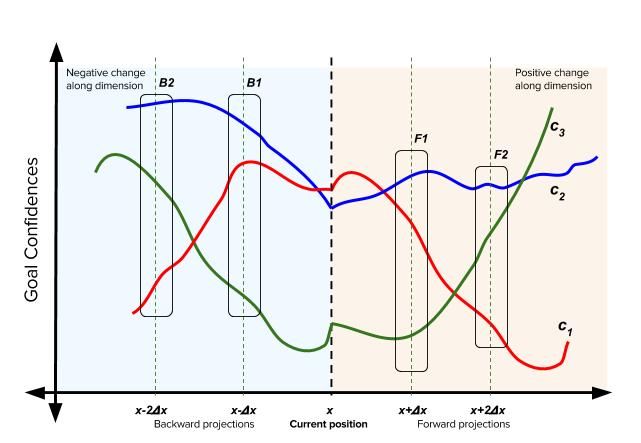
\includegraphics[width = 0.85\hsize, height = 0.45\vsize]{./figures/DisambMetric.jpg}
	\caption{In this example, $n_g = 3$. Furthermore, the region accessible due to a positive and negative change in the coordinate from the current position is shaded beige and light blue respectively. Additionally, the figure also shows a discontinuity in the confidences at the current position.}
	\label{DM_FIG}
\end{figure*}
\section{ALGORITHM DESIGN} \label{ALGO}
This section describes the algorithm that is used to compute the control mode with maximum confidence disambiguation, thereby eliciting the most legible control command from the human. Section~\ref{NOT} outlines the mathematical notation used and Section~\ref{DM} describes the different components that inform the confidence disambiguation metric. The details of the underlying blending based shared control system is also described briefly in this Section~\ref{BP}

\subsection{Notation}\label{NOT}

%Let $g_i \in \mathcal{G} \;\; \forall \;\;i \in [1,2,\dots,n_g]$, denote the $n_g$ number of possible goals in the scene and $c_i \in \mathcal{C} \;\; \forall \;\;i \in [1,2,\dots,n_g]$ denote the confidence that the system has in each one of the $n_g$ goals.

Let $\mathcal{G}$ be the set of all candidate goals in the scene with $n_g = \vert\mathcal{G}\vert$ and let $g^{i}$ refer to the $i^{th}$ goal where $i \in [1,2,\dots,n_g]$. The set of goals results in an associated set of confidences denoted as $\mathcal{C}$ and $c^{i}$ will refer to the individual confidence associated with goal $g^{i}$. Let $\mathcal{K}$ be the control space in which the robot operates and $k^{j}$ refer to an individual control dimension where $j \in [1,2,\dots,n_k]$.  The cardinality of $\mathcal{K}$ depends on the robotic platform, for example, for a smart wheelchair $n_k = 2$ (heading and forward velocity) whereas for a 6 DOF robotic arm $n_k = 6$.
%Let $\mathcal{G}$ be the set of all candidate goals in the scene with $\vert\mathcal{G}\vert = n_g$, resulting in an associated distribution of confidences $c_g \in \mathcal{C} \;\;( \forall \; g \in \mathcal{G})$  over candidate goals. Let $\mathcal{K}$ be the control space in which the robot operates with $\vert\mathcal{K}\vert = n_k$.
For control purposes, the set $\mathcal{K}$ is partitioned into subsets known as \textit{modes}. Let $\mathcal{M}$ refer to the set of all modes that the control space $\mathcal{K}$ is partitioned into with $n_{cm} = \vert\mathcal{M}\vert$. The number of modes ($n_{cm}$) is specific to the control interface and mapping. Furthermore, let $m^{p}$ refer to the $p^{th}$ mode where $p \in [1,2,\dots,n_{cm}]$.

Another quantity of interest is the gradient of individual goal confidences along the different control dimensions. More specifically, $\frac{\partial c^i}{\partial k^j}$ captures the rate of change of the confidence $c^{i}$ along control dimension $k^{j}$. Furthermore, since the confidence function, in general, can assume drastically different values upon moving in positive and negative directions along a control dimension, the left and right gradients are explicitly denoted as $\frac{\partial c^i}{\partial k^j}^{+}$ and $\frac{\partial c^i}{\partial k^j}^{-}$ respectively. The specific form of the confidence function used in our study will be discussed in Section~\ref{BP}, but the formalism developed in Section~\ref{DM} is agnostic to a particular form of confidence function. Additionally, an analytical closed-form expression for the gradient might not always be available as the confidence functions need not be continuous and differentiable. In other cases, due to the complexity of the confidence such an expression might be incredibly hard to compute. Therefore in our work, we numerically approximate the gradient by forward and backward differencing. 
%Lastly, we define a \textit{disambiguation} metric $D_{k_j}\in \mathbb{R}\; \forall \;k_j \in \mathcal{K}$ and is a function of the individual goal confidences $c_i$ and $\frac{\partial c_i}{\partial k_j}$\footnote{For the rest of the paper $\frac{\partial c_i}{\partial k_j}$ will be denoted as $ \dot{c}_{ij}$}. 

We define a \textit{disambiguation} metric  $D_{k^j}\in \mathbb{R}\; \forall \;k^j \in \mathcal{K}$ which is a function of $c^i$ and $\frac{\partial c^i}{\partial k^j}$\footnote{For the rest of the paper $\frac{\partial c^i}{\partial k^j}$ will be denoted as $ \dot{c}^{i}_j$}. Analogous to the gradients we explicitly define disambiguation metrics for both positive and negative directions as $D_{k_j}^{+}$ and $D_{k_j}^{-}$ respectively.

Lastly, we also define a disambiguation metric $D_m \in \mathbb{R}$ for each control mode $m \in \mathcal{M}$.
The disambiguation metric $D_m$ is a measure of how legible the user commands would be if the user were to control the robot in mode $m$. The higher the value, the easier it will be for the system to infer the human intent. 

\subsection{Disambiguation metric}\label{DM}
Let $\boldsymbol{x}$ be the current position of the robot in the world frame and the component of $\boldsymbol{x}$ along control dimension $k^j$ will be denoted as $x_{j}$. 
Figure~\ref{DM_FIG} is an illustrative example which shows how goal confidences can vary as a function of the position along a control dimension. 

The disambiguation metric $D_{k^j}$ encodes different aspects of how the goal confidences change upon moving (either in the positive or negative direction) along control dimension $k^j$. A proper design of $D_{k^j}$ should take into account both immediate as well as long term benefits of moving in $k^j$ and combine them into one metric. We identify four important considerations to  inform the design of $D_{k^j}$.

\subsubsection{Variance in confidences}
A good measure for evaluating the confidence disambiguation potential of a control dimension is to compute the ``variance'' ($SC^{\pm}_{k^j}$) in goal confidences. At any point in space this can be computed as the \textit{sum of pairwise distances} between the $n_g$ confidences. Since we are interested in the spread after a small change in position (due to user--initiated robot motion), we can sample the confidence function at $x_{k^j}\pm\Delta x_{k^j}$ and use the sampled values to compute $SC^{\pm}_{k^j}$, where $\Delta x_{k^j}$ is small change along the control dimension.
\begin{equation*}
SC^{\pm}_{k^j} = \sum_{p=1}^{n_g}\sum_{q=p}^{n_g}\norm{c^{p}_{x_{k^j} \pm \Delta x_{k^j}} - c^{q}_{x_{k^j} \pm \Delta x_{k^j}} }
\end{equation*}
\subsubsection{Mean of confidences}
The mean of the goal confidences is a good measure of the system's overall certainty in accurately estimating human intent. A higher mean implies that the system has a better idea of and is fairly sure of what the human is trying to do. The mean ($M^{\pm}_{k^j}$) is computed as
\begin{equation*}
M^{\pm}_{k^j} = \frac{\sum_{p = 1}^{n_g}c^{p}_{x_{k^j}\pm\Delta x_{k^j}}}{n_g}
\end{equation*}
\subsubsection{Difference between largest confidences}
For the blending paradigm, the current goal ($\boldsymbol{g}^{*}$) is the one with the highest confidence value. That is, 
\begin{equation*}
\boldsymbol{g}^{*} = g^{\argmax_i c^i}
\end{equation*}

Therefore, it is crucial that the difference between the largest and the second largest confidences in $\mathcal{C}$ is significant so that the computation of $\argmax_i c^i$ is unambiguous. Any ambiguity will likely result in a less accurate prediction of $\boldsymbol{g}^*$. This difference will be denoted by $D^{\pm}_{k^j}$ and is computed as
\begin{equation*}
D^{\pm}_{k^j} = max(c^{i}_{x_{k^j}\pm\Delta x_{k^j}}) - secondmax(c^{i}_{x_{k^j}\pm\Delta x_{k^j}})
\end{equation*}
\textbf{[Need better notation for this. Can't think of one right now.]}
\subsubsection{Gradients}
The propensity for change and information gain upon the continuation of motion along control dimension $k^j$ is encoded in the gradients $\frac{\partial c^i}{\partial k^j}\; \forall\; c^i\in \mathcal{C}$. The greater the difference between the gradients of individual confidences $c^i$, the greater will they deviate from each other. This would indicate to the system that something ``interesting'' might happen if the motion is continued along the control dimension. Instead of using closed form analytical gradients, we approximate the gradients using forward and backward differences. Therefore, 
\begin{equation*}
\frac{\partial c^i}{\partial k^j}^{\pm} \approx c^{i}_{x_{k^j} \pm 2\Delta x_{k^j}} - c^{i}_{x_{k^j} \pm \Delta x_{k^j}} 
\end{equation*}
In order to quantify the ``spread'' of gradients we define a quantity $SD^{\pm}_{k^j}$ which is computed as 
\begin{equation*}
SD^{\pm}_{k^j} = \sum_{p=1}^{n_g}\sum_{q=p}^{n_g}\norm{\frac{\partial c^i}{\partial k^j}^{+} - \frac{\partial c^i}{\partial k^j}^{-}}
\end{equation*}

\subsubsection*{Putting it all together}
$SC^{\pm}$, $M^{\pm}$, $D^{\pm}$ and $SD^{\pm}$ are then combined to compute $D_{k^j}^{\pm}$ as 
\begin{equation*}
D_{k^j}^{\pm} = \underbrace{\boldsymbol{w}_1(SC^{\pm}\cdot M^{\pm} \cdot D^{\pm})}_{\text{long term}} + \underbrace{(1 - \boldsymbol{w}_1)\cdot SD^{\pm}}_{\text{short term}}
\end{equation*}
where $\boldsymbol{w}_1$ controls the relative contribution of immediate and the long term benefit. 
Once $D_{k^j}^{\pm}$ is computed $D_{k^j}$ and $D_m$ can be evaluated as 
\begin{equation*}
D_{k^j} = D_{k^j}^{+} + D_{k^j}^{-}
\end{equation*}
\begin{equation*}
D_m = \sum_{j} D_{k^j} \; \forall \; k^j \in m
\end{equation*}
Thus, the mode with highest disambiguation capability $\boldsymbol{m}^{*}$ is given by
\begin{equation*}
\boldsymbol{m}^* = \argmax_m D_m
\end{equation*}
$\boldsymbol{m}^{*}$ is the mode that the algorithm chooses \textit{for} the human upon assistance request. Any subsequent control command issued by the user in $\boldsymbol{m}^*$ is likely to the more legible due to maximal goal confidence disambiguation.

\subsection{Blending paradigm}\label{BP}
\begin{wrapfigure}[12]{R}{0.27\textwidth}
	\begin{center}
		\vspace{-.6cm}
		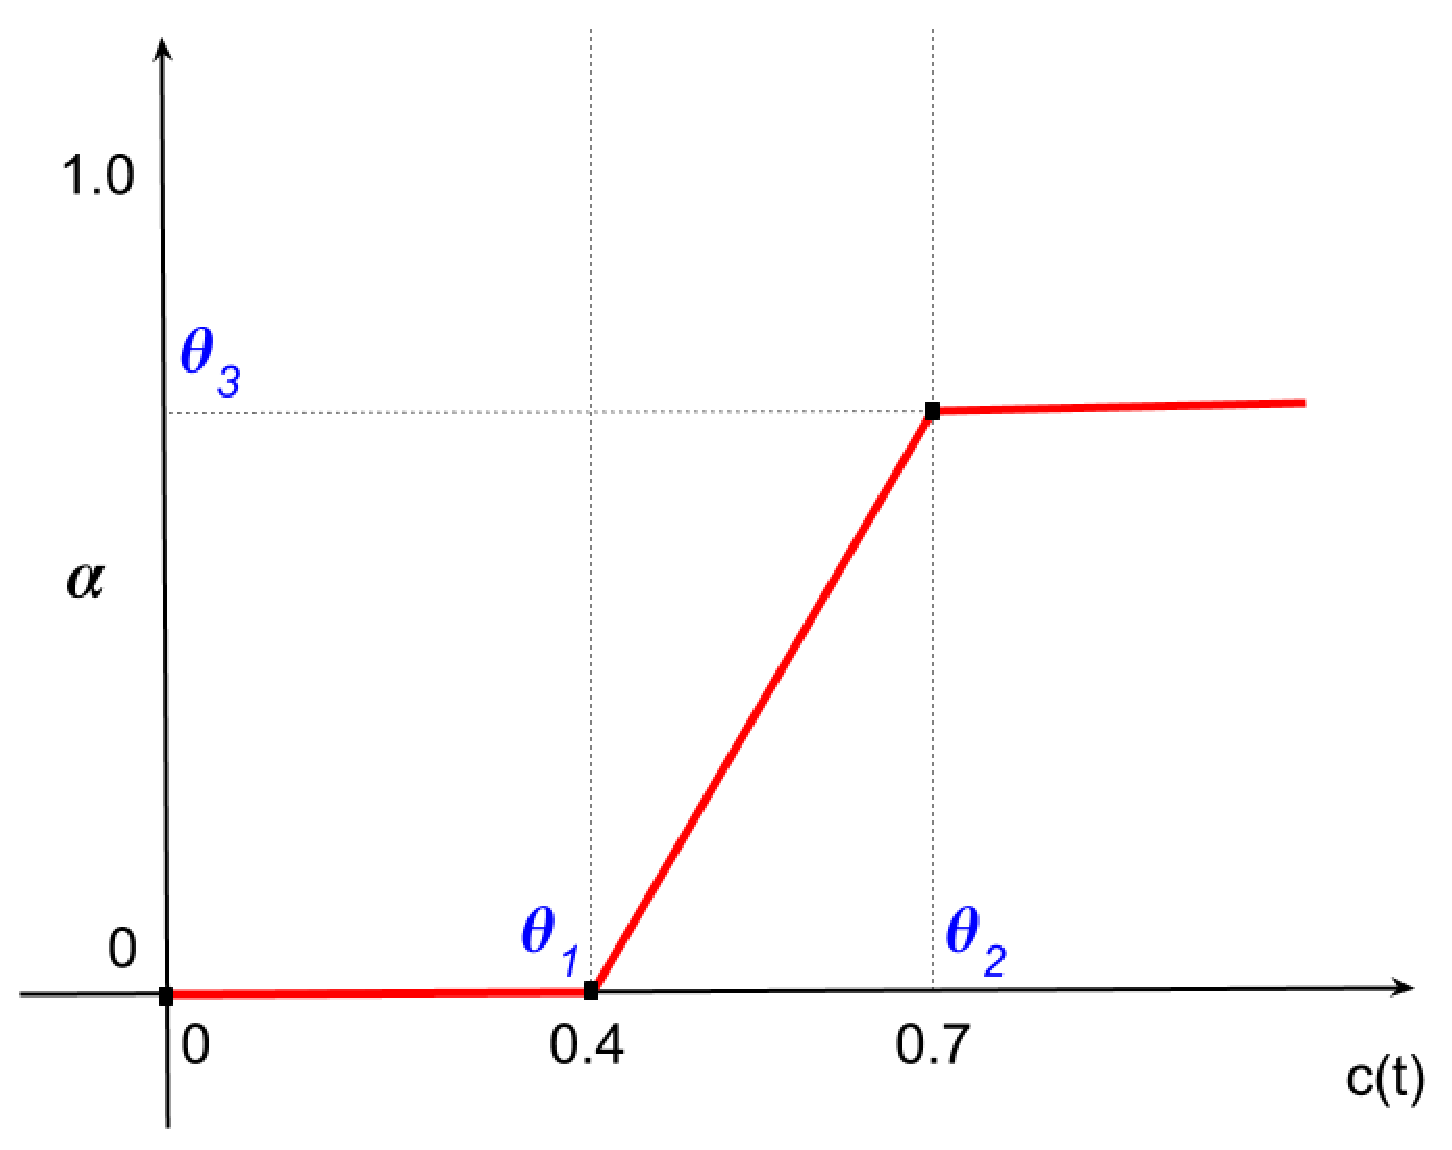
\includegraphics[width=0.27\textwidth]{./figures/Figure2.eps}
	\end{center}
		\vspace{-.45cm}
	\caption{A prototypical arbitration function, parameterized by {\footnotesize $\boldsymbol{\theta} = \{\theta_{1}, \theta_{2}, \theta_{3}\}$}.}
	\label{ALPHA}
\end{wrapfigure}
The proposed mode switching assistance paradigm augments a blending based shared control system in which the final control command issued to the robot is a blended sum of the human control command and an autonomous robot policy. The blending factor ($\alpha$) is a function of the system confidence in its own estimate of the human intent. 

Let $\boldsymbol{u}_h$ be the human control command and $\boldsymbol{u}_{r}^{i}$ be the autonomous control policy associated with goal $g^i$. The final control command $\boldsymbol{u}_f$, issued to the robot is then given as 
\begin{equation*}
\boldsymbol{u}_f = \alpha\cdot \boldsymbol{u}_r^{i^*} + (1 - \alpha)\cdot \boldsymbol{u}_h
\end{equation*}
where $i^{*}$ is the index associated with $\boldsymbol{g}^{*}$.

In our implementation $c^i$ is computed as
\begin{equation}\label{E1}
c^i = (\boldsymbol{u}_h \cdot \boldsymbol{u}_r^i)_{trans} + (\boldsymbol{u}_h \cdot \boldsymbol{u}_r^i)_{rot}
\end{equation}

The first and the second terms in Equation~\ref{E1} captures the alignment between the human control command and the autonomous robot policy in the translational and rotational parts of the state space respectively. 
The blending factor $\alpha$ is a parameterized function of the confidence and is depicted in Figure~\ref{ALPHA}.

The robot control command $\boldsymbol{u}_r$ is generated using a simple potential field based dynamical system which is defined in all parts of the state space. Every goal $g^i$ is associated with a potential field $P^{i}$ which treats $g^i$ as an attractor and all the other goals in the scene as repellers. For potential field $P^i$, the attractor velocity is given by
\begin{equation*}
\dot{\boldsymbol{x}}^i_{attract} = \boldsymbol{x}_{g^i} - \boldsymbol{x}
\end{equation*}
where $\boldsymbol{x}_{g^i}$ is the location of $g^i$ and the repeller velocity
\begin{equation*}
\dot{\boldsymbol{x}}^i_{repel} = \sum_{p} \frac{\boldsymbol{x} - \boldsymbol{x}_{g^p}}{\eta(\norm{\boldsymbol{x} - \boldsymbol{x}_{g^p}}^2)}
\end{equation*}
where $p \in \{1,2,\dots,n_g\} \setminus \{i\}$. Additionally, $P^i$ operates in full six dimensional Cartesian space. 

\section{STUDY METHODS} \label{EXP}
\subsection{Hardware}
\subsubsection{Robotic Platform}
The experiments were performed using the MICO robotic arm (Kinova Robotics, Canada) which is a 6 DOF robotic arm specifically designed for assistive purposes. The software system was implemented using the Robot Operating System (ROS) and data analysis was performed using MATLAB. 
\subsubsection{Control Interfaces}
In our experiments, the human control command $\boldsymbol{u}_h$ was captured using two different control interfaces: 2-axis joystick (J2) and a head array (HA). 

A 2-axis joystick (shown in Figure blah) generates continuous signals and is capable of controlling a maximum of two control dimensions at a time. Different control modes can be accessed using the buttons on the interface. 

On the other hand, a head array is a switch based discrete teleoperation device. The head array consists of three switches; the switch at the back is used to cycle between the modes and the switches on the left and right side are to control the motion in the positive and negative direction along a control dimension. 
	\begin{table}
	\centering
	\begin{tabular}{|l|c|c|}
		\hline
		\multicolumn{3}{|c|}{Control Mappings} \\
		\hline
		\textbf{Mode} & \textbf{HA} & \textbf{J2}\\
		\hline
		1 & $v_{x}$ & $v_{x}, v_{y}$ \\ \hline
		2 & $v_{y}$   & $v_{x}, v_{z}$ \\ \hline
		3 & $v_{z}$ &  $\omega_{z}, \omega_{y}$ \\ \hline
		4 & $\omega_{z}$   & $\omega_{x}$ \\ \hline
		5 &  $\omega_{y}$  & ---  \\ \hline
		6 & $\omega_{x}$   & ---  \\ \hline
	\end{tabular}
	\vspace{.2cm}
	\caption{Operational paradigms for the teleoperation interfaces} 
	\label{CIM}
	\vspace{-.5cm}
\end{table}

The control interface signals are mapped to Cartesian velocities of the end effector of the robot and the mappings used by both interfaces are shown in Table~\ref{CIM}. Additionally, the interfaces can also be used to request mode switch assistance. 

\subsection{Task Descriptions}
\noindent\underline{\textit{Simple Reaching}}: The user operates the robotic arm using both control interfaces to perform simple reaching motions to two different goal locations. This is a training task and the primary purpose is to get the user accustomed to the operation of the control interfaces. 

\noindent\underline{\textit{Reaching with same grasp (RsG)} }: The user teleoperates the robotic arm using both control interfaces to perform reaching motions towards one of the four objects on the table with the same grasp orientation. The table top set up is shown in the middle column of Figure blah. 

\noindent\underline{\textit{Reaching with different grasp (RdG)}}: This is a more difficult task that \textit{RsG} in which the user operates the robot to perform reaching motions to one of the five objects in the scene with different grasp orientations. This setup is shown in the right most column of Figure blah. 

Analysis was performed only on data collected from \textit{RsG} and \textit{RdG}. 

\subsection{Assistance Paradigms}
Three kinds of mode switching assistance paradigms were tested in this study. 

\noindent\underline{\textit{Without assistance}}: In this paradigm, only the blending based system is at work and the user is free to operate in any mode he/she wants. 

\noindent\underline{\textit{With assistance}}: In this paradigm, the mode switch system is activated right at the beginning of a trial. The algorithm returns the ``best mode'' $\boldsymbol{m}^*$ and places the human in control mode $\boldsymbol{m}^*$ afterwards which the human will perform the tasks. At any stage during task execution the user is still allowed to change modes, if needed. 

\noindent\underline{\textit{Free exploration}}: In free exploration, the user is free to execute the task in any way he/she wants and the mode switch assistance system is always available. The user can request a mode switch assistance any time during the course of task execution. This paradigm is exploratory and seeks to find underlying patterns in assistance request behavior. 
\subsection{Study Protocol and Metrics}
\noindent\underline{\textit{Subjects}}: For this study 10 subjects were recruited. Fill in details. 

\noindent\underline{\textit{Protocol}}:
A within-subject study was conducted using a full factorial design in which the manipulated variables are the tasks, control interfaces and assistance paradigms. The study consisted of two phases. In phase I, each user performed both tasks, using both interfaces with and without assistance. The trials were balanced and the tasks, control interfaces and the paradigms were randomized to eliminate ordering effects. The starting positions of the robot and the initial mode of operation were also randomized to avoid biases. Three trials were collected for each permutation of manipulated variables.  
In phase II, the user performed the same tasks using both interfaces using the \textit{free exploration} paradigm. 

\noindent\underline{\textit{Metrics}}: A number of objective metrics were evaluated during this study. \textit{Task completion time} is the amount of time a user spends in accomplishing a task. \textit{Mode switches} refer to the number of times the user switched between various modes while performing the task and is an indicator of effort. Subjective evaluation was also performed at the end of the trials in which the user was required to answer a post experiment questionnaire containing questions regarding the utility value, system's accuracy in estimating human intent and user acceptance. 

\section{RESULTS AND DISCUSSION} \label{RES}
\section{CONCLUSIONS}\label{CON}


%\subsection{Subsection Heading Here}
%Subsection text here.
%
%\subsubsection{Subsubsection Heading Here}

%
%
%\section{RSS citations}
%
%Please make sure to include \verb!natbib.sty! and to use the
%\verb!plainnat.bst! bibliography style. \verb!natbib! provides additional
%citation commands, most usefully \verb!\citet!. For example, rather than the
%awkward construction 
%
%{\small
%\begin{verbatim}
%\cite{kalman1960new} demonstrated...
%\end{verbatim}
%}
%
%\noindent
%rendered as ``\cite{kalman1960new} demonstrated...,''
%or the
%inconvenient 
%
%{\small
%\begin{verbatim}
%Kalman \cite{kalman1960new} 
%demonstrated...
%\end{verbatim}
%}
%
%\noindent
%rendered as 
%``Kalman \cite{kalman1960new} demonstrated...'', 
%one can
%write 
%
%{\small
%\begin{verbatim}
%\citet{kalman1960new} demonstrated... 
%\end{verbatim}
%}
%\noindent
%which renders as ``\citet{kalman1960new} demonstrated...'' and is 
%both easy to write and much easier to read.
%  
%\subsection{RSS Hyperlinks}
%
%This year, we would like to use the ability of PDF viewers to interpret
%hyperlinks, specifically to allow each reference in the bibliography to be a
%link to an online version of the reference. 
%As an example, if you were to cite ``Passive Dynamic Walking''
%\cite{McGeer01041990}, the entry in the bibtex would read:
%
%{\small
%\begin{verbatim}
%@article{McGeer01041990,
%  author = {McGeer, Tad}, 
%  title = {\href{http://ijr.sagepub.com/content/9/2/62.abstract}{Passive Dynamic Walking}}, 
%  volume = {9}, 
%  number = {2}, 
%  pages = {62-82}, 
%  year = {1990}, 
%  doi = {10.1177/027836499000900206}, 
%  URL = {http://ijr.sagepub.com/content/9/2/62.abstract}, 
%  eprint = {http://ijr.sagepub.com/content/9/2/62.full.pdf+html}, 
%  journal = {The International Journal of Robotics Research}
%}
%\end{verbatim}
%}
%\noindent
%and the entry in the compiled PDF would look like:
%
%\def\tmplabel#1{[#1]}
%
%\begin{enumerate}
%\item[\tmplabel{1}] Tad McGeer. \href{http://ijr.sagepub.com/content/9/2/62.abstract}{Passive Dynamic
%Walking}. {\em The International Journal of Robotics Research}, 9(2):62--82,
%1990.
%\end{enumerate}
%%
%where the title of the article is a link that takes you to the article on IJRR's website. 
%
%
%Linking cited articles will not always be possible, especially for
%older articles. There are also often several versions of papers
%online: authors are free to decide what to use as the link destination
%yet we strongly encourage to link to archival or publisher sites
%(such as IEEE Xplore or Sage Journals).  We encourage all authors to use this feature to
%the extent possible.
%
%\section{Conclusion} 
%\label{sec:conclusion}
%
%The conclusion goes here.

\section*{Acknowledgments}

%% Use plainnat to work nicely with natbib. 

\bibliographystyle{plainnat}
\bibliography{references}

\end{document}


